\chapter{2D LIDAR Feature Extraction for SLAM}
\label{cha:featureExtractors}
To improve the estimate of the state and to get an idea of our environment, the input of the exteroceptive sensors has to be analyzed. As seen in chapter \ref{cha:Platform }, the robot is equipped with both a Camera and a 2D scanning LIDAR.

\section{Feature Extraction with Point Features}
\label{sec:spike}
\subsection{Overview}
 In this section a simple algorithm is used to detect fixed features in the environment. The algorithm is mainly based on large jumps in the range measurement of the LIDAR. The algorithm is then improved using preexisting knowledge of the environment.

\subsection{Feature Extraction Algorithm}
\label{sec: spikeAlgo}
Consider an extremely clean environment. One which has only fixed features and they are all away from the wall. And the entire environment is within the range of the LIDAR. In such an environment the distance readings gradually increase and decrease all along the walls except when they encounter and obstacle or a \textit{feature}. This algorithm essentially looks for large jumps in the distance readings. One such arena is shown in Figure~\ref{fig:Simulated_1}. The gradual nature of the distance readings are more clearly seen when the scan values are plotted as a function of the angle of the scan beam with respect to the robot as shown in Figure~\ref{fig:Vrep_plot}.
\begin{figure}[h!]
    \centering
    \begin{subfigure}[b]{0.3\textwidth}
    
	    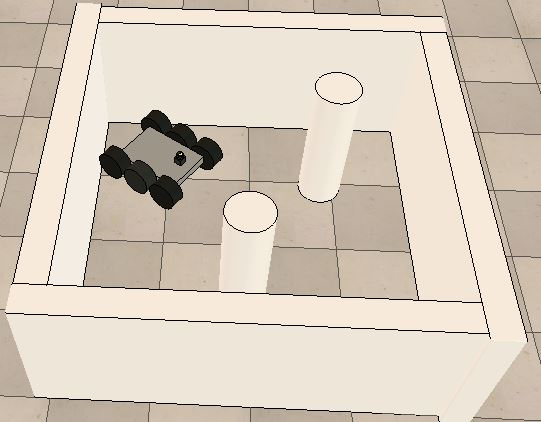
\includegraphics[width=\textwidth]{3d_vrep}
	    \caption{A simulated arena.}
	    \label{fig:3d_vrep}
    \end{subfigure}
    \quad %add desired spacing between images, e. g. ~, \quad, \qquad, \hfill etc.
      %(or a blank line to force the subFigure~onto a new line)
    \begin{subfigure}[b]{0.3\textwidth}
        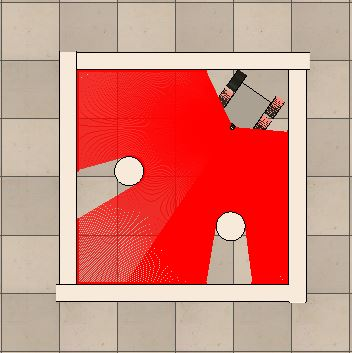
\includegraphics[width=\textwidth]{arena_vrep}
        \caption{Top view.}
        \label{fig:arena_vrep}
    \end{subfigure}%
        \caption{Simulated arena for LIDAR.}
        \label{fig:Simulated_1}
\end{figure}

For the robot to detect the large jumps the distance is differentiated with respect to angles. As seen in Figure~\ref{fig:Vrep_cylinders} this will give a specific pattern each time a cylinder is present. A condition can then be designed in the following way. Each time the derivative is larger than a fixed threshold and is a negative number, a cylinder's beginning is found, and when a large positive value is encountered, it's end. Finding the mid point of these two readings the location of the cylinder is found as in Figure~\ref{fig:Vrep_cylinders}. 
\begin{figure}
        \centering

        \begin{subfigure}[b]{0.48\textwidth}
                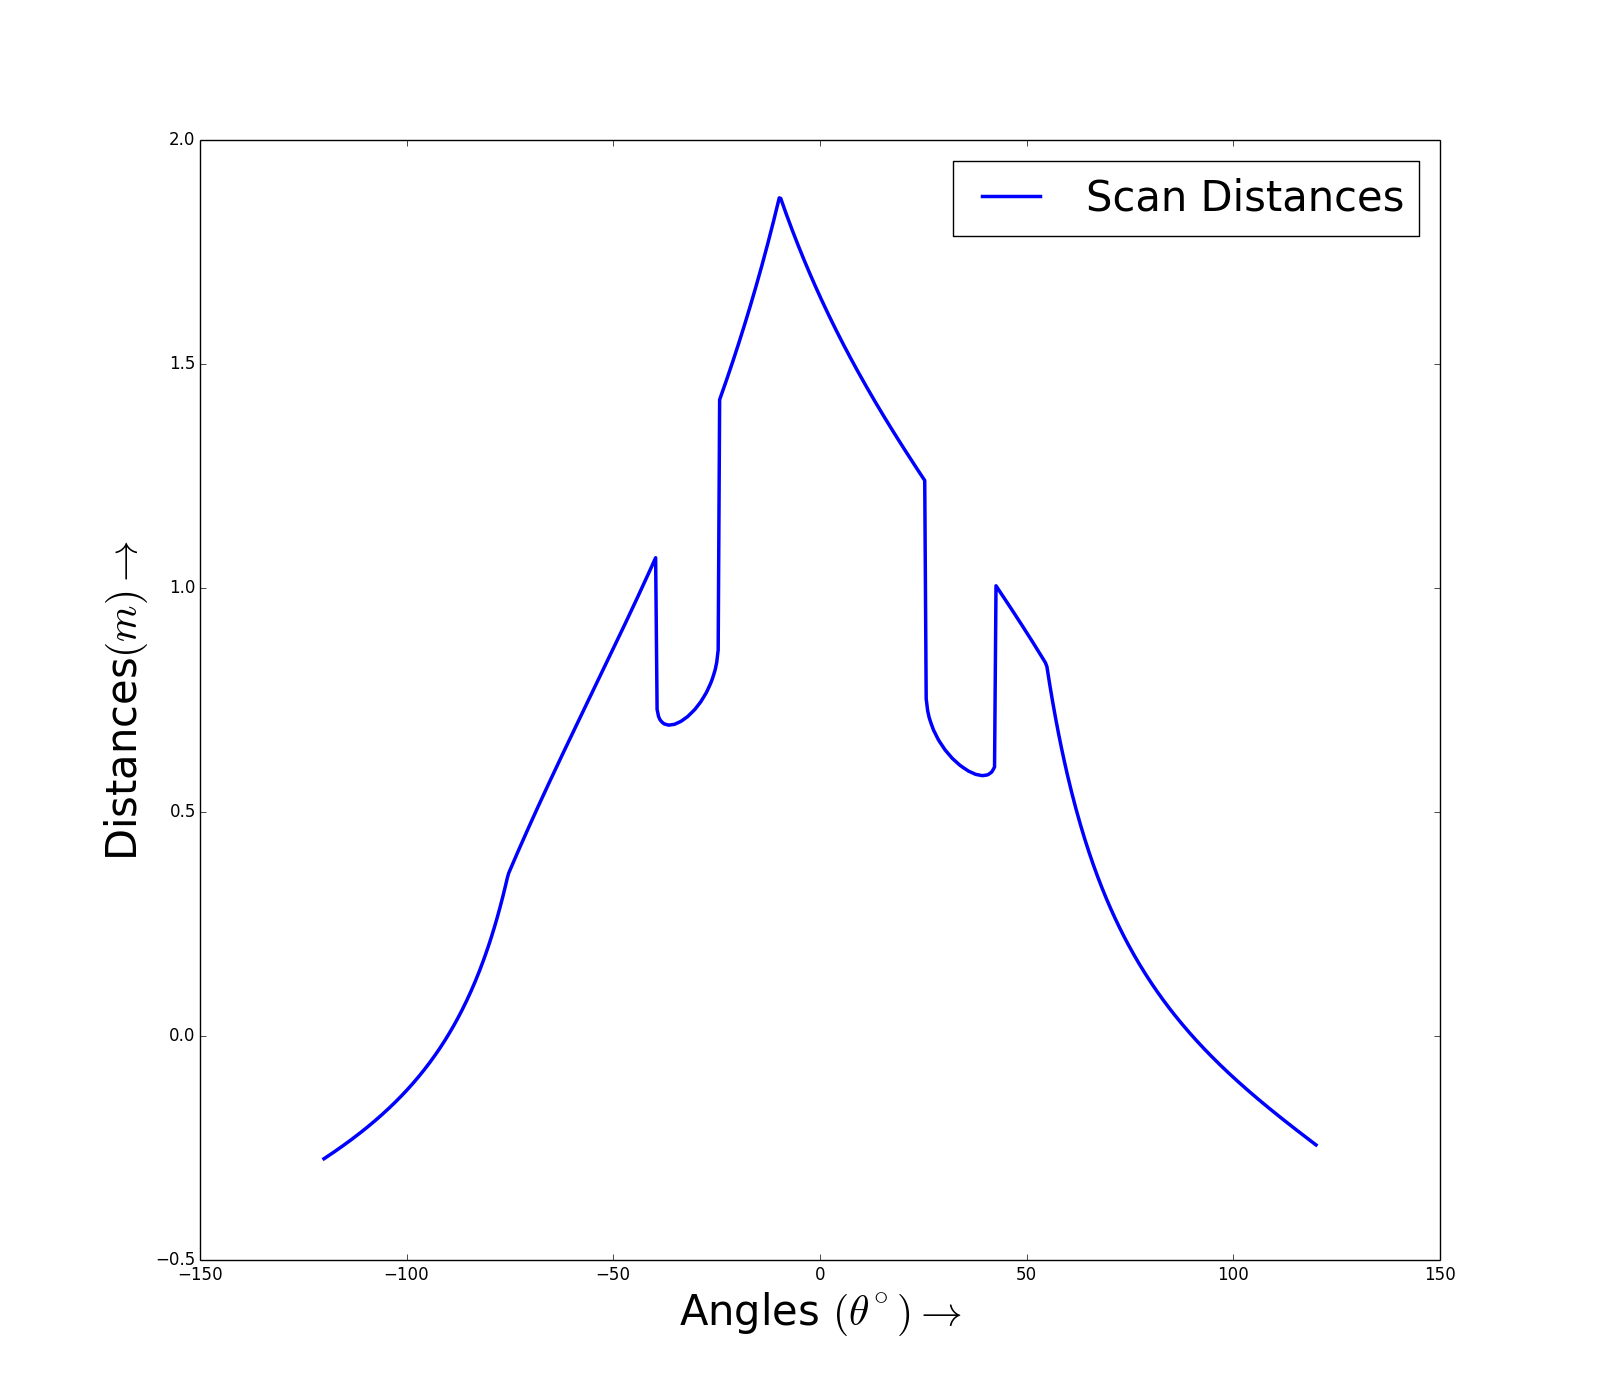
\includegraphics[width=\textwidth]{Vrep_plot}
                \caption{LIDAR scan.}
                \label{fig:Vrep_plot}
        \end{subfigure}
        \quad %add desired spacing between images, e. g. ~, \quad, \qquad, \hfill etc.
          %(or a blank line to force the subFigure~onto a new line)
%        \begin{subfigure}[b]{0.3\textwidth}
%                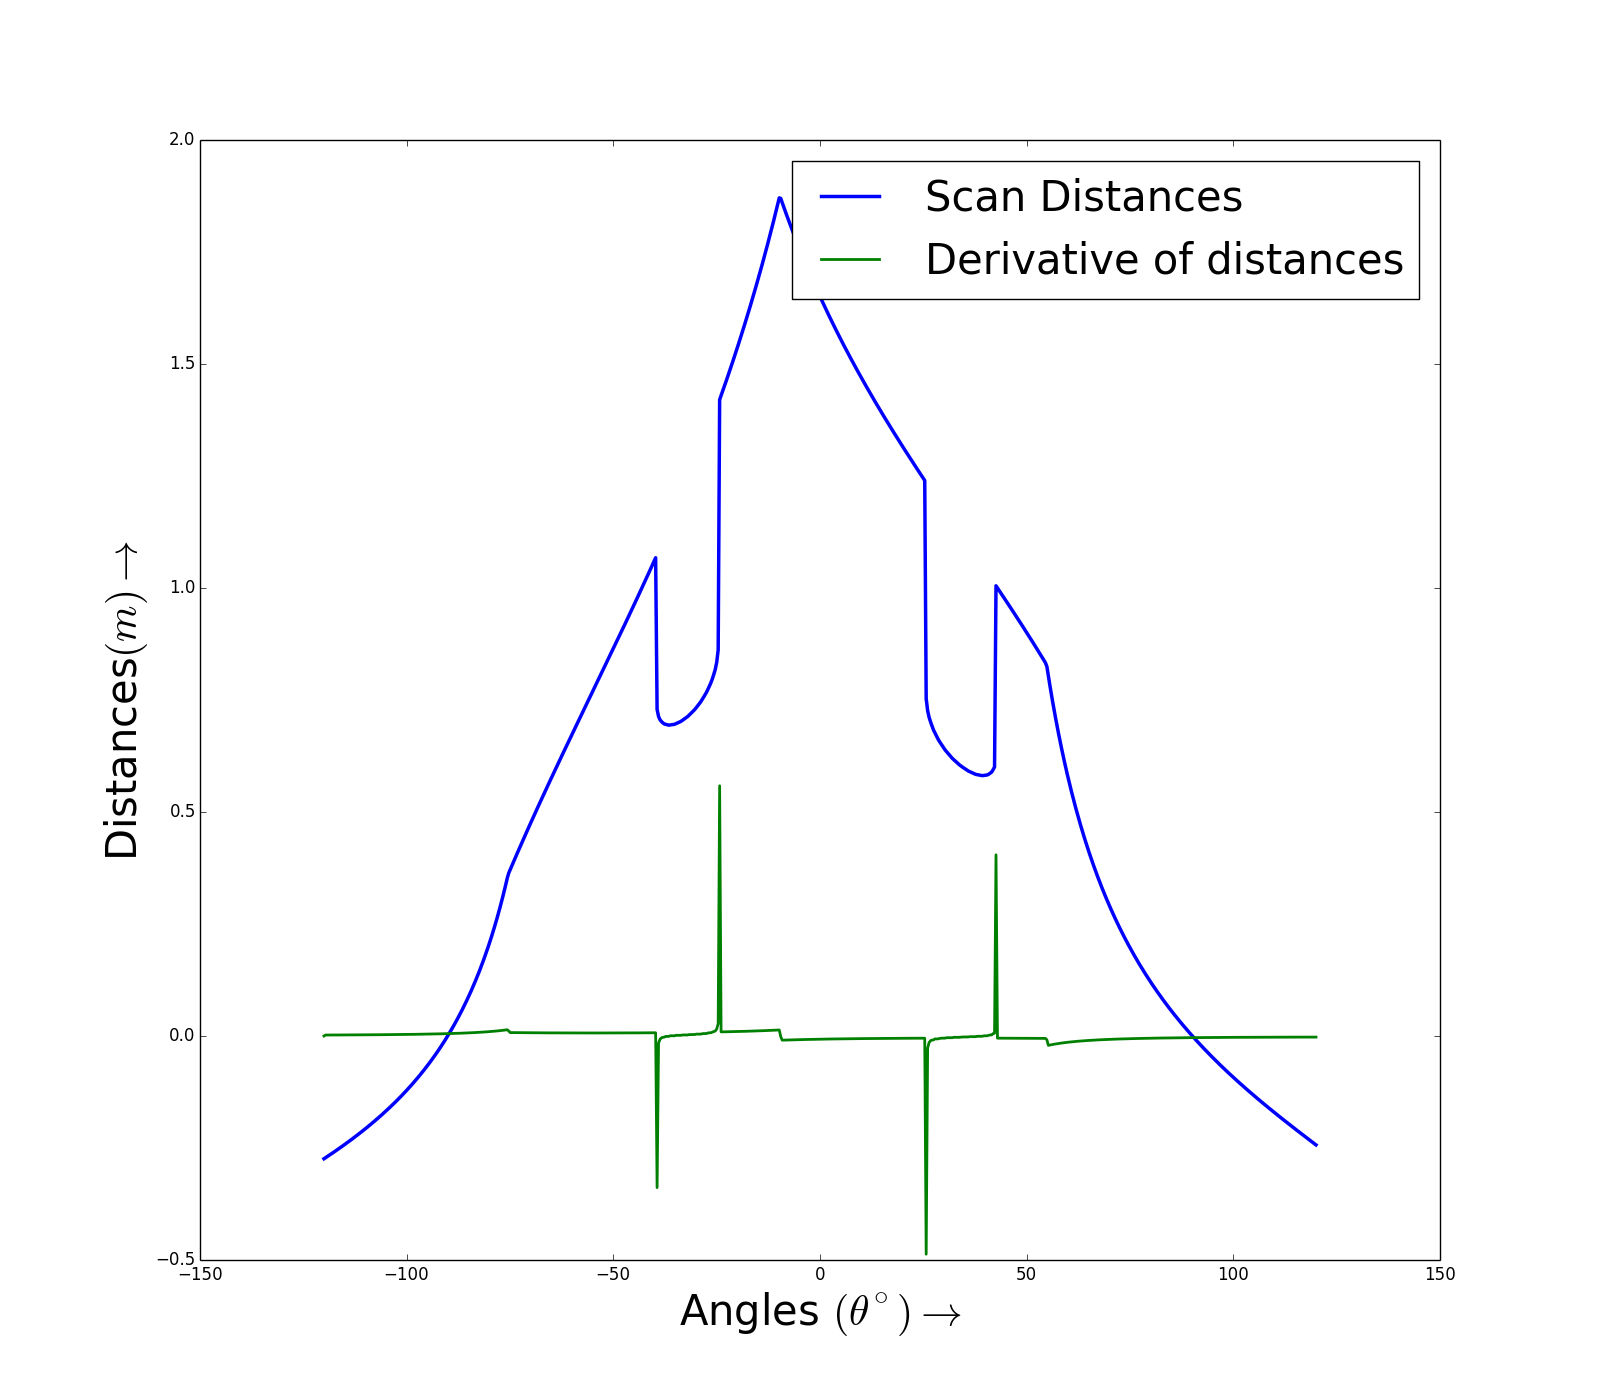
\includegraphics[width=\textwidth]{Vrep_derivative}
%                \caption{Derivative of scan}
%                \label{fig:Vrep_derivative}
%        \end{subfigure}%
        \quad %add desired spacing between images, e. g. ~, \quad, \qquad, \hfill etc.
          %(or a blank line to force the subFigure~onto a new line)
        \begin{subfigure}[b]{0.48\textwidth}
                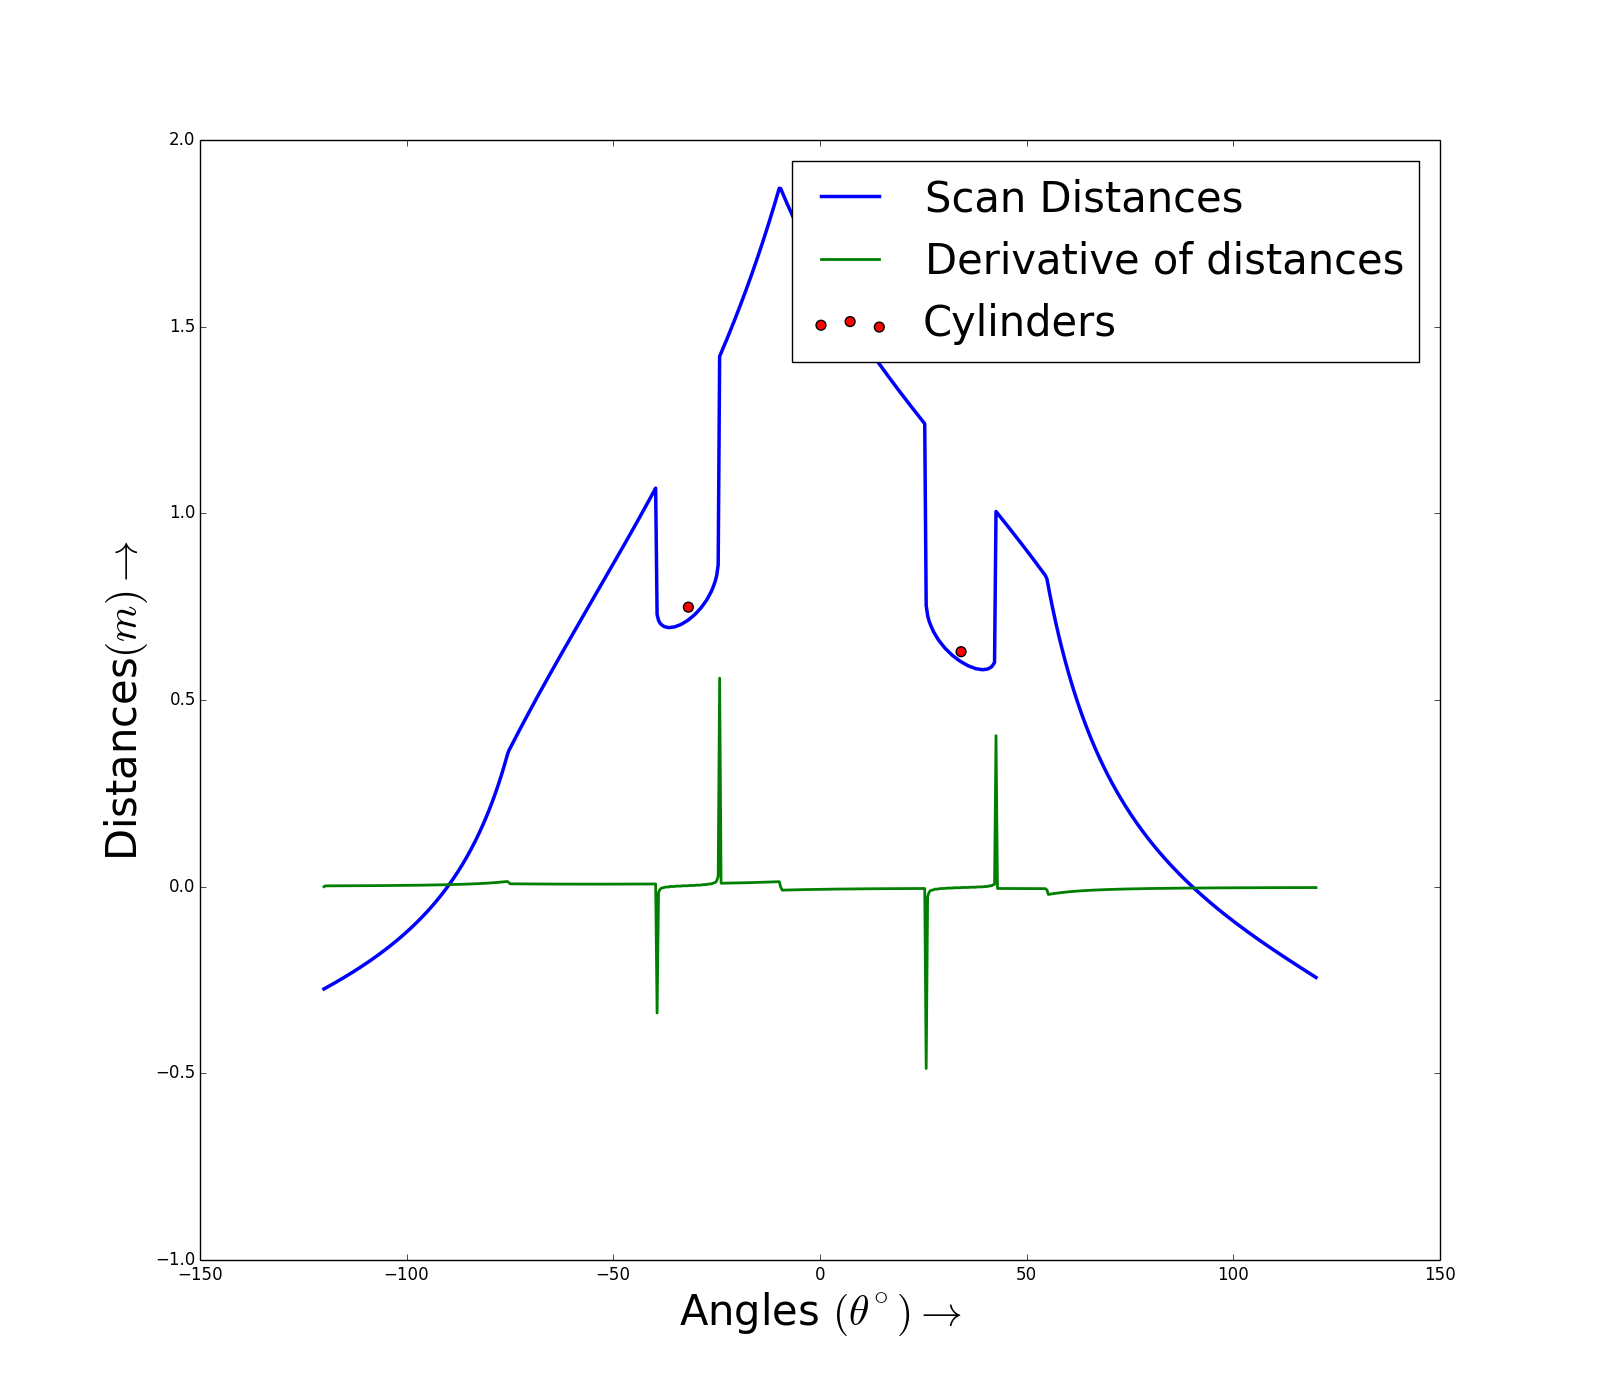
\includegraphics[width=\textwidth]{Vrep_cylinders}
                \caption{Detected cylinders.}
                \label{fig:Vrep_cylinders}
        \end{subfigure}

        \caption{Differential based LIDAR feature detection}\label{fig:Simulated_2}
\end{figure}

It is apparent this method has a large number of drawbacks. The arena has to be fully within the range of the sensor, if not there will be breaks in the distance curve that will generate spurious landmarks. This drawback can be easily overcome by creating a zero order hold for those regions. Also any disturbances in the boundaries will also generate spurious landmarks. The threshold for the derivative is a very sensitive tuning parameter. If it is set too high there is an increased chance of missing landmarks placed closed to walls and if it is set low, there are a large number of spurious landmarks. 

To overcome this, based on preexisting knowledge of the nature of features a filter of sorts can be designed. A low threshold is chosen and a large number of prospective features are enumerated. All those that lack a minimum number of points on them are immediately eliminated. Next, based on the fact that the radius of the cylinders that are the landmarks is known, the angular width of any feature detected can be approximated. From the large set, only the ones within a range around this approximate angular width are retained. Then, the least squares fit is computed to check if the features are indeed cylinders or segments of the wall. Only the features having a large enough curvature are retained. By this method a small amount of robustness is added to a simplistic algorithm of feature detection. The results of such a filter when applied with EKF can be seen in section \ref{sec:Spike_results}.

Once the features are detected, the measurement model from the robot to these features need to be calculated to be used in \ekf SLAM.

\subsection{Examples}
\label{sec:Spike_results}

In a clean simulated arena the results of the first approach is seen in section \ref{sec: spikeAlgo}. But in a real world environment, a large number of variations will occur. To demonstrate this a relatively clean real world environment is considered as shown in Figure~\ref{fig:Real world arena} The zero values are caused by the entire arena not being within the range of the LIDAR. 
\begin{figure}[h!]
    \centering
    \begin{subfigure}[b]{0.45\textwidth}
    
	    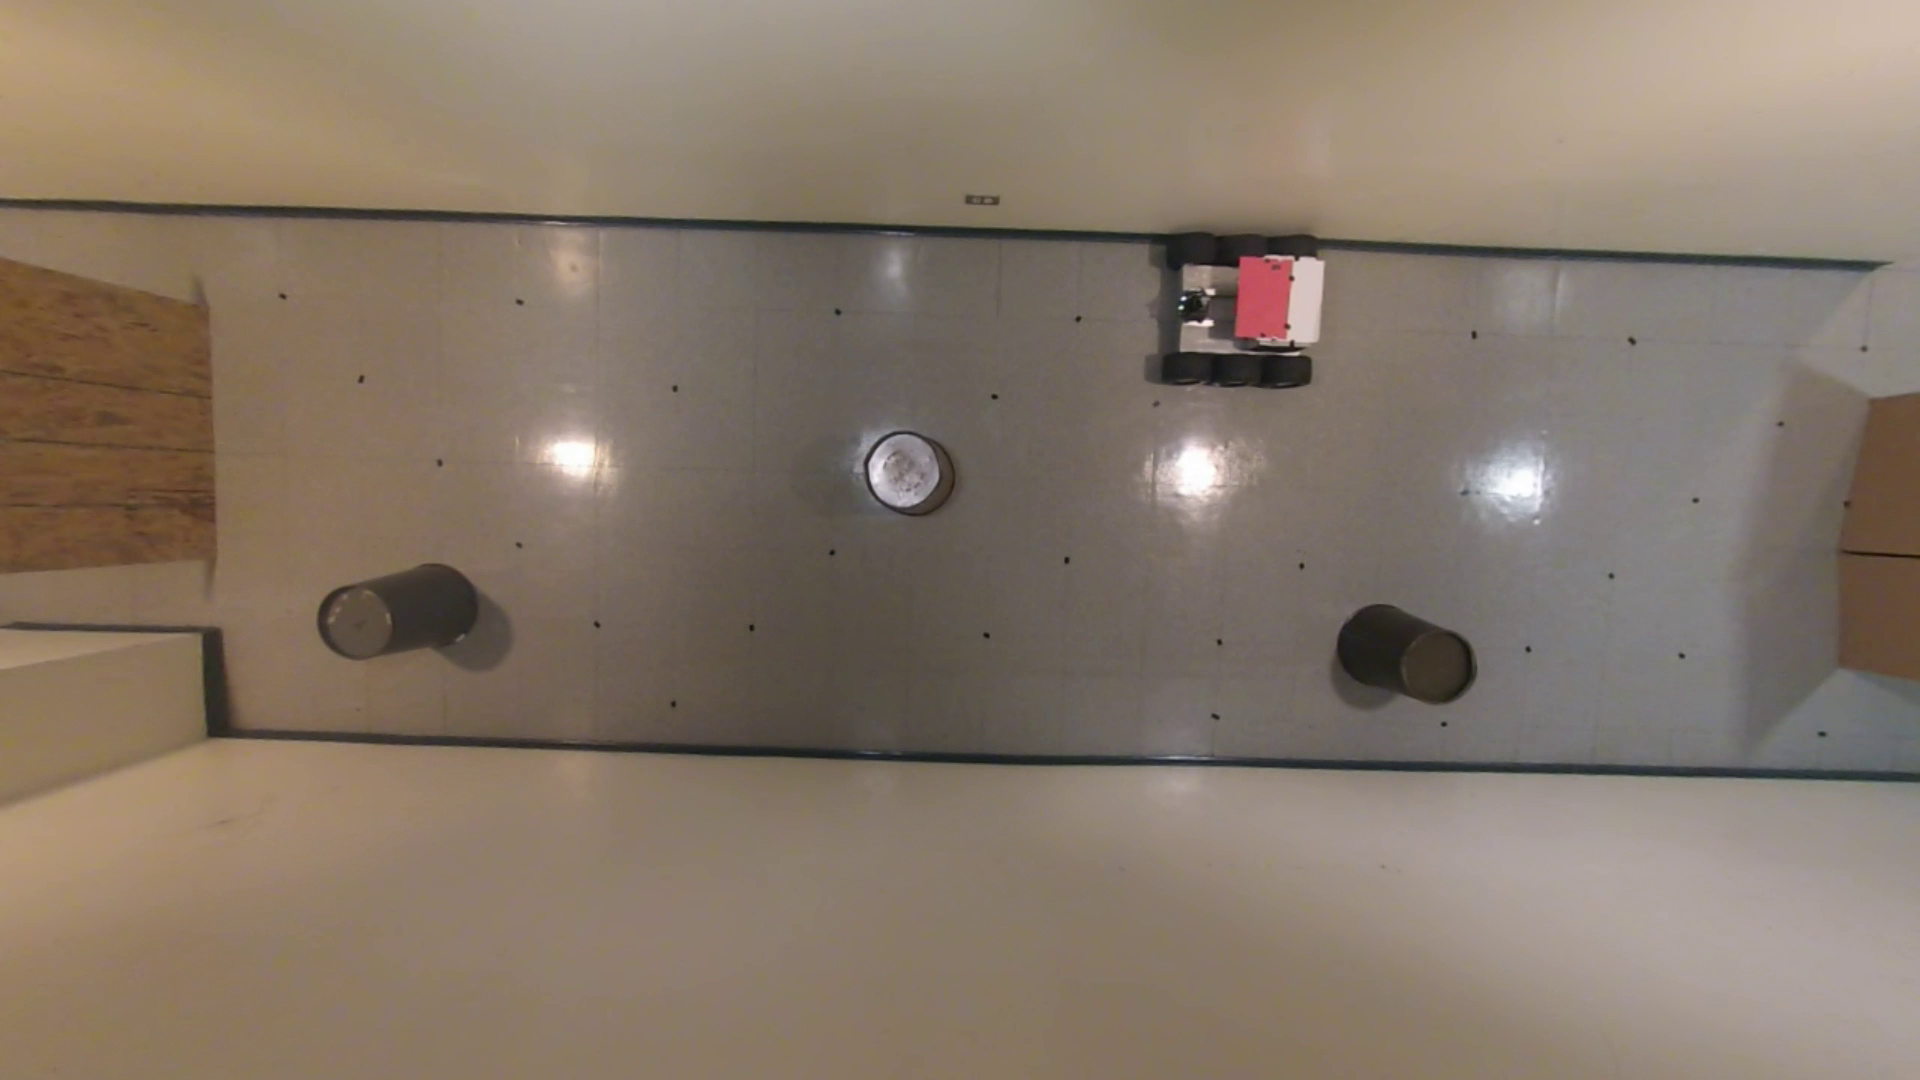
\includegraphics[width=\textwidth]{overhead}
	    \caption{Overhead view.}
	    \label{fig:overhead}
    \end{subfigure}
    \quad %add desired spacing between images, e. g. ~, \quad, \qquad, \hfill etc.
      %(or a blank line to force the subFigure~onto a new line)
    \begin{subfigure}[b]{0.45\textwidth}
        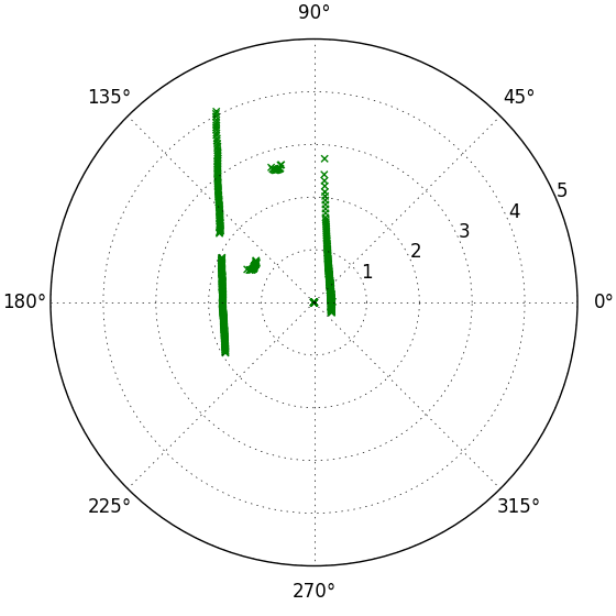
\includegraphics[width=\textwidth]{blank_scan}
        \caption{Polar plot of laser scan.}
        \label{fig:spike_scan}
    \end{subfigure}%
        \caption{Real world arena.}
        \label{fig:Real world arena}
\end{figure}

With such an arena if just jumps in distance are used to determine the cylinder position a large number of spurious landmarks are detected as shown in Figure~\ref{fig:Spike_cylinders_bad}. These cannot be avoided by simply changing the threshold for the change in derivative. It is possible to avoid some by interpolating the data whenever the distance is zero, but this introduces additional problems when the robot is too close to an obstacle and if a landmark is too close to a wall. 

\begin{figure}[h!]
    \centering
    \begin{subfigure}[b]{0.45\textwidth}
	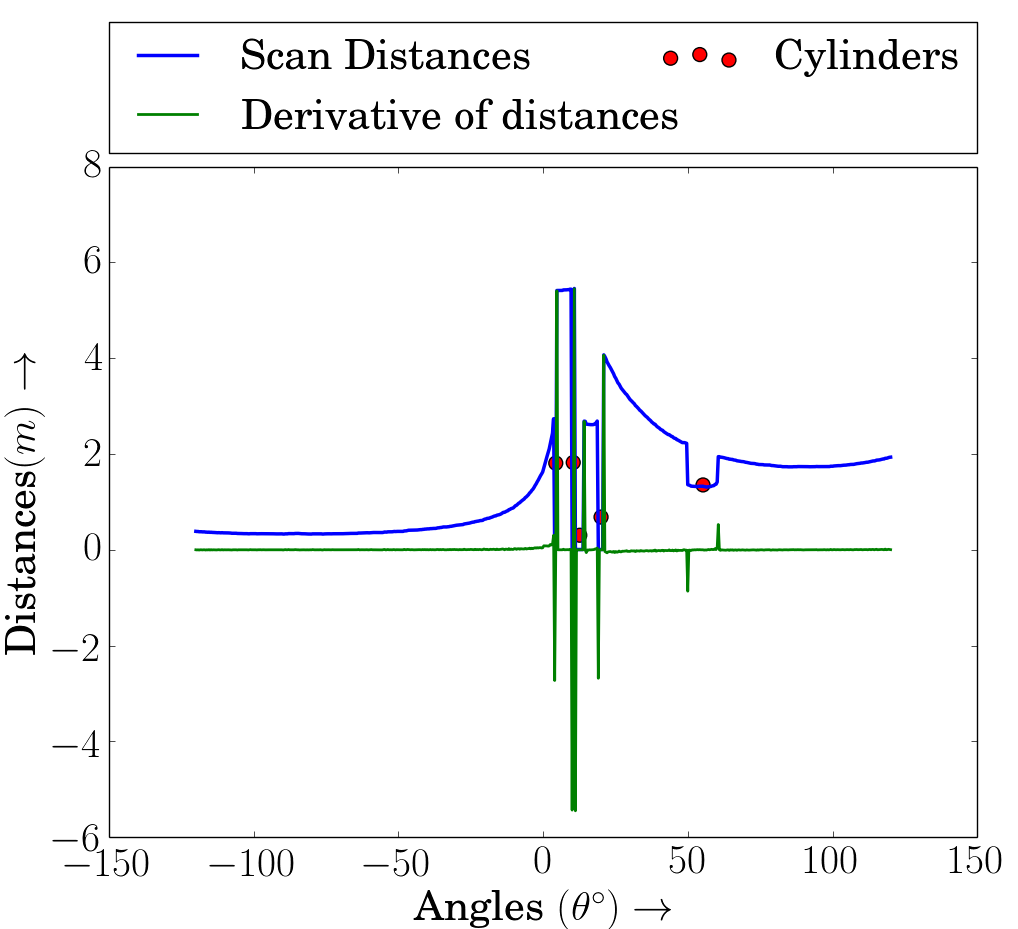
\includegraphics[width=\textwidth]{spike_cyl_bad}
    \end{subfigure}
    \quad %add desired spacing between images, e. g. ~, \quad, \qquad, \hfill etc.
      %(or a blank line to force the subFigure~onto a new line)
    \begin{subfigure}[b]{0.45\textwidth}
        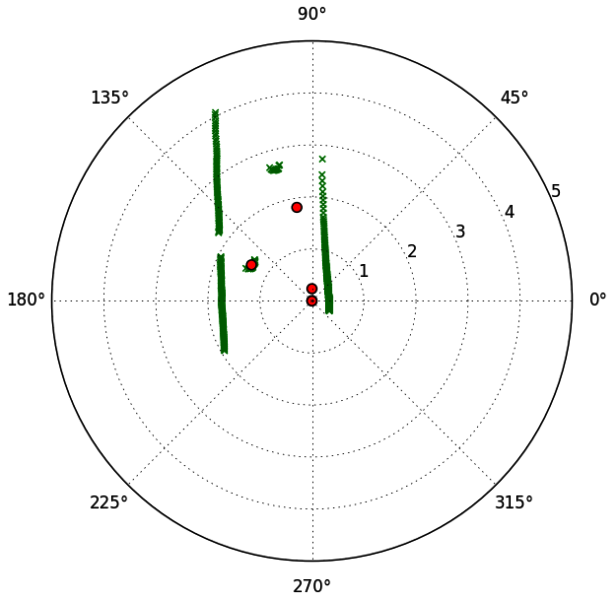
\includegraphics[width=\textwidth]{spike_cyl_badPol}
    \end{subfigure}%
	\caption{Spurious cylinders detected in data.}
	\label{fig:Spike_cylinders_bad}
\end{figure}

\begin{figure}[h!]
\centering
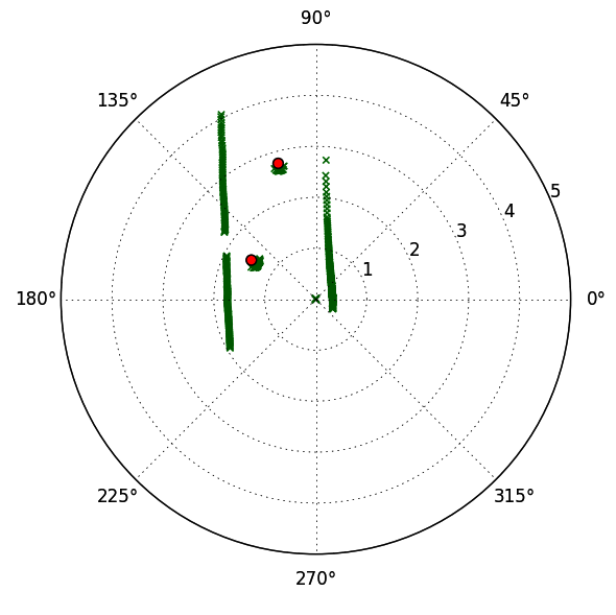
\includegraphics[width=0.4\textwidth]{spike_good}
\caption{After filtering of candidate cylinders.}
\label{fig:spike_good}
\end{figure}

To refine this conditions similar to those discussed in section \ref{sec: spikeAlgo} are implemented. This is seen to give much better results. as seen in Figure~\ref{fig:spike_good}. 



\subsection{Measurement Model and the corresponding Jacobian matrices}
\label{sec:Spike_math}

Once the cylinder coordinates are found in the LIDAR data, it's position has to be stored in the map.  Since an estimate of the robot's position in the inertial frame is known, the cylinder coordinates are mapped from robot to inertial frame using a homogeneous transformation as in Equation~\ref{eq:SpikeMath1}. Where $ (x_w,y_w) $ are coordinates in world frame. $ (x_r,y_r,\theta_r) $ are estimated pose of the robot and $ (x_1,y_1) $
\begin{equation}
\begin{bmatrix}
x_w\\y_w\\1
\end{bmatrix}=
\begin{bmatrix}
\cos(\theta_r) & -\sin(\theta_r) & x_r\\
\cos(\theta_r) & \sin(\theta_r) & y_r\\
0 & 0 & 1
\end{bmatrix}
\begin{bmatrix}
x_1\\y_1\\1
\end{bmatrix}
\label{eq:SpikeMath1}
\end{equation}

Once the cylinder is in inertial frame the next step is to check if it corresponds to any preexisting cylinder in the map. For this the euclidean distance between the detected cylinder and the existing cylinder positions is measured and if it is less than a particular threshold then the new cylinder is associated with the existing one. 

For the correction of the robot pose as explained in section \ref{sec:EKF_SLAM}, the measurement model of the point features is needed. That is a mapping that gives the laser reading or the distance $ r $ and angle $ \alpha $ from the robot to the cylinder. For this first the coordinates of the cylinder in the robots frame of reference is found using the inverse of the homogeneous transformation in Equation~\ref{eq:SpikeMath1}. But the robot pose used now is the new position at this particular time step. Once $ (x_1,y_1) $ is found in the robot frame, the measurement h can be found using Equation~\ref{eq:SpikeMath2}. The same equations are used for every the corresponding cylinder that is detected to give $ z $ which is used to calculate the \textit{innovation} in Equation~\ref{eq:EKF_8}.

\begin{equation}
	\label{eq:SpikeMath2}
	h=\begin{bmatrix}
	r\\\alpha
	\end{bmatrix}=
	\begin{bmatrix}
	\sqrt{(y_1-y_r)^2+(x_1-x_r)^2} \\
	\tan^{-1}\left(\frac{y_1-y_r}{x_1-x_r}\right)-\theta_r
	\end{bmatrix}
\end{equation}

The measurement model gives the innovation but not the Kalman Gain. For this, according to Equation~\ref{eq:EKF_7} the derivatives of the model with respect to the state vector $ x \in \Re^n $ is used. The state contains both the robot pose as well as all the landmarks already existing in the map at that particular time step. Since it is assumed each landmark is independent of the other, most part of the Jacobian $ H $ contains zeros except for the part corresponding to the robot pose and if the measurement has been associated with an existing landmark, then it will depend on that landmark's position. Hence for the Jacobian $ H $, the measurement model $ h $ is differentiated as per Equation~\ref{eq:SpikeMath3}. 

\begin{equation}
\label{eq:SpikeMath3}
	H = 
	\begin{bmatrix}
	\frac{\partial r}{\partial x_r} & \frac{\partial r}{\partial y_r} & \frac{\partial r}{\partial \theta_r} & \cdots & \frac{\partial r}{\partial x_1} & \frac{\partial r}{\partial y_1} & \cdots \\
	\frac{\partial \alpha}{\partial x_r} & \frac{\partial \alpha}{\partial y_r} & \frac{\partial \alpha}{\partial \theta_r} & \cdots & \frac{\partial \alpha}{\partial x_1} & \frac{\partial \alpha}{\partial y_1} & \cdots 
	\end{bmatrix}
\end{equation}

Each of the terms are derived separately as per Equation~\ref{eq:SpikeMath4}. 

\begin{subequations}
\label{eq:SpikeMath4}
	\begin{align}
	\frac{\partial r}{\partial x_r} &= \frac{(x_r-x_1)}{\sqrt{(y_1-y_r)^2+(x_1-x_r)^2}} \qquad
	\frac{\partial \alpha}{\partial x_r} =  
	\frac{(y_1-y_r)}{(y_1-y_r)^2+(x_1-x_r)^2} \\
	\frac{\partial r}{\partial y_r} &= \frac{(y_r-y_1)}{\sqrt{(y_1-y_r)^2+(x_1-x_r)^2}} \qquad
	\frac{\partial \alpha}{\partial y_r} =  
	\frac{(y_r-y_1)}{(y_1-y_r)^2+(x_1-x_r)^2} \\
	\frac{\partial r}{\partial \theta_r} &= 0 \qquad  
	\frac{\partial \alpha}{\partial \theta_r} = -1\\
	\frac{\partial r}{\partial x_1} &= \frac{(x_r-x_1)}{\sqrt{(y_1-y_r)^2+(x_1-x_r)^2}} \qquad
	\frac{\partial \alpha}{\partial y_1} =  
	\frac{(y_1-y_r)}{(y_1-y_r)^2+(x_1-x_r)^2} \\
	\frac{\partial r}{\partial x_1} &= \frac{(y_r-y_1)}{\sqrt{(y_1-y_r)^2+(x_1-x_r)^2}} \qquad
	\frac{\partial \alpha}{\partial y_1} =  
	\frac{(y_r-y_1)}{(y_1-y_r)^2+(x_1-x_r)^2}	
	\end{align}
\end{subequations}

The only other information needed for Kalman Gain calculation is the observer error $ V^TRV $ with V being the derivative of the measurement model with respect to noise. If all landmarks are assumed to be uniformly affected by noise, it is reasonable to approximate V to be an identity matrix. R is the measurement noise. It is a diagonal matrix with one of the eigenvalues representing the error in distance measurement of the LIDAR and the other the angle measurement as in Equation~\ref{eq:SpikeMath5}. 
\begin{equation}
\label{eq:SpikeMath5}
R = 
\begin{bmatrix}
\sigma_r & 0 \\
0 & \sigma_\alpha
\end{bmatrix}
\end{equation}

Using all this information, as in it is possible to correct the estimate of the robot pose while simultaneously correcting the position of the landmarks. The result of such a \slam is seen in section...